% !TeX encoding = UTF-8
% !TeX spellcheck = fr_FR
\documentclass[french,12pt,a4paper,titlepage,openright,openbib]{report}

\usepackage[utf8]{inputenc}
\usepackage[T1]{fontenc}
\usepackage[french]{babel}
\usepackage[default]{gillius}

\usepackage{graphicx}
\usepackage{lipsum}
\usepackage{array}
\usepackage[pdfborder={0 0 0}]{hyperref}
\usepackage[xindy,toc]{glossaries}
\usepackage{titlesec}
\usepackage{color}
\usepackage{blindtext}
\usepackage{fancyhdr}
\usepackage{lastpage}
\usepackage[pages=some]{background}
\usepackage[pass]{geometry}
\usepackage{afterpage}
\usepackage{emptypage}
\usepackage{fancybox}


% !TeX encoding = UTF-8
% !TeX spellcheck = fr_FR
% !TeX root = RapportMi3A.tex

%defini le style de couverture
\fancypagestyle{couverture}{
	\fancyhf{}
	\renewcommand \headrulewidth{0pt}
	\renewcommand \footrulewidth{0pt}
}

%default header & footer
\fancyhf{}
%redefinition du footer
\fancyfoot[C]{Page \textbf{\thepage} sur \textbf{\pageref{LastPage}}}
\renewcommand \footrulewidth{0pt}

%definition du header
\fancyhead[L]{\raisebox{-0.2 \height}{
\includegraphics[width=2cm]{logo_nxp}}}
\fancyhead[R]{\textsc Rapport de mi-parcours 3A}
\renewcommand \headrulewidth{0pt}

%colors
\definecolor{gray75}{gray}{0.75}
\definecolor{aqua}{RGB}{0,164,167}
\definecolor{petrol}{RGB}{0,112,136}

\definecolor{nxpblue}{RGB}{123,177,219}
\definecolor{nxporange}{RGB}{249,181,0}
\definecolor{nxpgreen}{RGB}{201,210,0}

\parindent=0in
\parskip=8pt

%margins 1 inch
\addtolength{\oddsidemargin}{-.5in}
\addtolength{\evensidemargin}{-.5in}
\addtolength{\textwidth}{1.2in}

\addtolength{\topmargin}{-.5in}
\addtolength{\textheight}{0.8in}

%ajoute une page blanche
\newcommand{\blankpage}{%
	\null
	\thispagestyle{empty}%
	\addtocounter{page}{-1}%
	\newpage}
%ajouter un hespace de 20pt
\newcommand{\hsp}{\hspace{20pt}}
%numérotaiton romaine
\renewcommand\thechapter{\Roman{chapter}}
\renewcommand\thesection{\Roman{section}}
\renewcommand \thesubsection {\thesection.\Roman{subsection}}

%modification du style de chapitre
\titleformat{\chapter}[hang]{\Huge\bfseries}{\thechapter\hsp\textcolor{gray75}{|}\hsp}{0pt}{\Huge\bfseries}
\titlespacing{\chapter}{0pt}{0pt}{12pt}

%Renomme Bibliogrphy en
%\renewcommand{\bibname}{Références}

%redefini le style plain qui est utilisé sur les premières pages de chapitre
\fancypagestyle{plain}{%
	\fancyhf{} % clear all header and footer fields
	\fancyfoot[C]{Page \textbf{\thepage} sur \textbf{\pageref{LastPage}}} % except the center
	\fancyhead[L]{\raisebox{-0.2 \height}{
\includegraphics[width=2cm]{logo_nxp}}}
	\fancyhead[R]{\textsc Rapport de mi-parcours 3A}
	\renewcommand \headrulewidth{0pt}
	\renewcommand{\footrulewidth}{0pt}}



\graphicspath{{template/}{img/}}

\title{Rapport de mi-parcours de troisième année}
\author{Jennifer Gr\"{a}nicher}
\date{12 février 2018}

\pagestyle{fancy}


\makeglossaries
\newglossaryentry{mifare}
{
	name=MIFARE,
	description={Marque de NXP incluant une large gamme de circuits intégrés sans contact},
}
\newglossaryentry{desfire}
{
	name=DESFire,
	description={Marque de la famille MIFARE qui permet de créer des systèmes de cartes sécurisées grâce à l'alliance de la cryptographie et du sans contact},
}
\newglossaryentry{mooc}
{
	name=MOOC,
	description={Massive Open Online Course, formation ou cours en ligne},
	plural=MOOCs
}
\newacronym{nfc}{NFC}{Near Field Communication}
\newacronym{jee}{JEE}{Java Entreprise Edition}

\begin{document}
% !TeX encoding = UTF-8
% !TeX spellcheck = fr_FR
% !TeX root = RapportMi3A.tex

\backgroundsetup{
	scale=1,
	color=black,
	opacity=1.0,
	angle=0,
	contents={%
		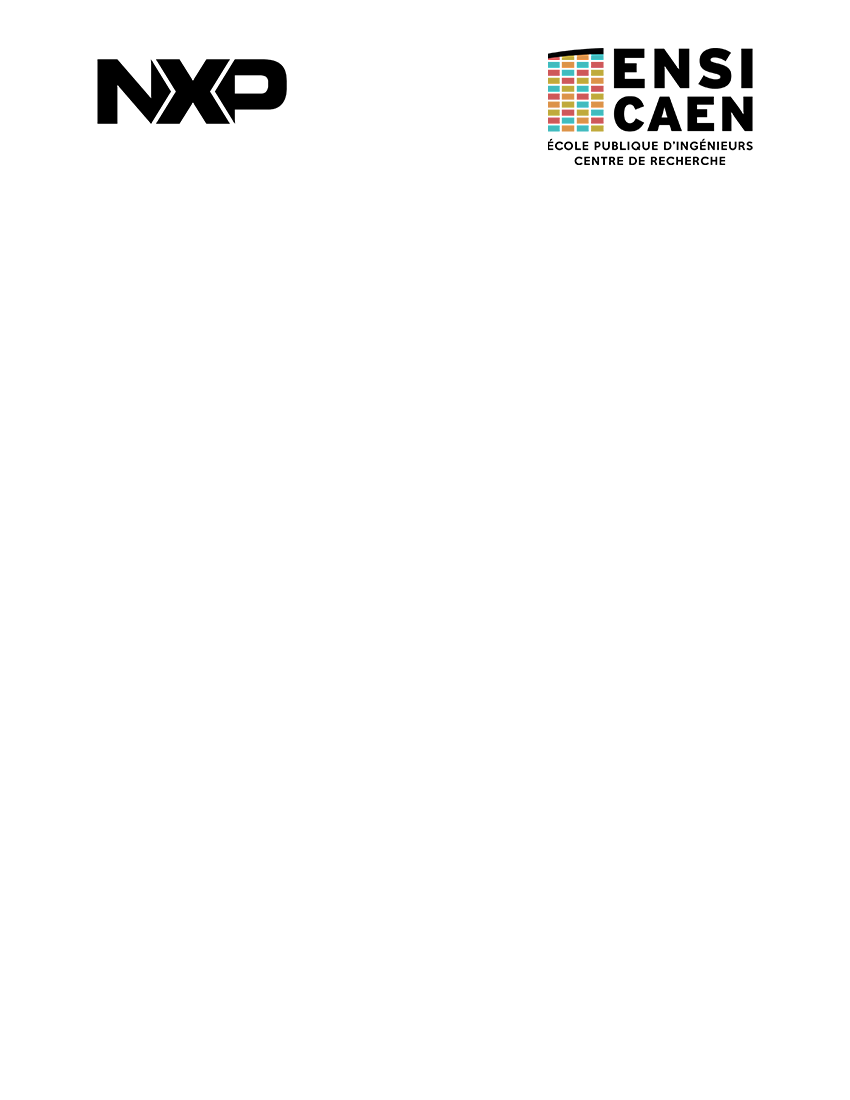
\includegraphics[width=\paperwidth, height=\paperheight]{cover_tmpl}
	}%
}

{
	\BgThispage
	\thispagestyle{couverture}
	
	\newgeometry{headheight=80pt, top=6cm, headsep=3cm}
	
	\makeatletter
	{\LARGE\bfseries\@title\par}
	{\color{aqua}Informatique par apprentissage \\
	\color{aqua}Année universitaire 2017-2018}
	\hfill
	\vspace{0.5cm}
	
	\includegraphics[width=15cm]{scylla}
	\vspace{0.5cm}
	
	\begin{minipage}[c]{0.5\textwidth}
	Tuteur école \par
	{\color{aqua} Wilfried \bsc{Aubry}}
	
	\vspace{0.5cm}
	
	Maître d'apprentissage \par
	{\color{aqua} Nicolas \bsc{Guillerm}}
	\end{minipage}
	\begin{minipage}[c]{0.5\textwidth}
	Tuteur école \par
	{\color{aqua} Wilfried \bsc{Aubry}}
	
	\vspace{0.5cm}
	
	Maître d'apprentissage \par
	{\color{aqua} Nicolas \bsc{Guillerm}}
	\end{minipage}
	
		
		
	
	\makeatother
	
	\vfill
	
	\afterpage{\blankpage}
	\restoregeometry
}


\maketitle

\chapter*{Remerciements}
J'aimerais remercier toutes les personnes qui ont contribué au bon déroulement de ces trois dernières années d'apprentissage, au sein de l'entreprise NXP Semiconductors, et au sein de l'ENSICAEN.

Je tiens particulièrement à remercier Virginie Jobard qui m'a épaulée et aidée à prendre mes repères au début.

Je souhaiterais également remercier Didier Graignic qui a su prendre le relais et m'aiguiller au cours de ma mission sur le projet MOOCTab \cite{website:mooctab} \cite{website:mooctabitea}.

J'aimerais aussi remercier Nicolas Guillerm pour toute l'aide qu'il a apporté que ce soit pour le rapport ou les missions au sein de l'entreprise.

Je remercie également Wilfried Aubry qui a été de bon conseil et qui a su apporter une grande aide.

Je tiens également à remercier mes collègues chez NXP pour leur aide et leur soutien.

\tableofcontents

\chapter*{Historique}
\begin{table}[ht]
	\label{tab:historique}
	\centering
	\begin{tabular}{|c|c|c|c|}
		\hline
		{\bf Version} & {\bf Date} & {\bf Rédigé par}    & {\bf Mise à jour}    \\
		\hline
		1.0           & 29/01/2018 & Jennifer Gränicher  & Création du document \\
		\hline
		1.1           & 06/02/2018 & Jennifer Gränicher  & Mise en page \\
		\hline
		1.1           & 12/02/2018 & Jennifer Gränicher  & Finalisation \\
		\hline
	\end{tabular}
\end{table}

\vspace{2cm}

{\let \clearpage \relax \chapter*{Diffusion}}
\begin{table}[ht]
	\label{tab:diffusion}
	\centering
	\begin{tabular}{|c|c|c|c|}
		\hline
		{\bf Destinataire} & {\bf Société}      & {\bf Fonction}   		 & {\bf Date}\\
		\hline
		Nicolas Guillerm   & NXP Semiconductors & Maitre d'apprentissage & 08/02/2018 \\
		\hline
		Wifried Aubry      & ENSICAEN 			& Tuteur				 & 12/02/2018 \\
		\hline
	\end{tabular}
\end{table}

\chapter{Introduction}
Ce document parle de mes trois années d'apprentissage au sein de NXP Semiconductors, de Septembre 2015 à Janvier 2018.

Une première partie concerne les derniers changements au sein de l'entreprise.
Une seconde traite des projets en cours, elle est centrée sur la dernière année.
Enfin, une autre partie traite de mon évolution personnelle et professionnelle au cours de ces trois années.

\chapter{Actualités}
Au cours des derniers mois les effectifs de NXP à Caen ont été réduits. Cela a eu pour conséquence un réaménagement de certains services.

Didier Graignic, qui remplaçait Virginie Jobard, a quitté l'entreprise. Nicolas Guillerm l'a remplacé en qualité de maître d'apprentissage.

L'équipe avec laquelle je travaille est aujourd'hui composée de Nicolas Guillerm, Dominique Défossez et moi-même. Dominique Défossez est responsable stratégie et partenariat pour NXP Semiconductors en France, il s'occupe notamment du management des projets européens.
Cette équipe travaille pour le compte de NXP sur le projet MOOCTab, que je détaillerai plus loin.
\section{Qualcomm}
En octobre 2016 Qualcomm annonçait son souhait de racheter NXP Semiconductors. La commission américaine avait approuvé ce rachat mais la commision européenne avait été saisie par une entreprise concurrente.

Après une enquête approfondie, la commission européenne a finalement accepté le rachat, uniquement sous certaines conditions :
Qualcomm n'acquerra pas les brevets essentiels au standard \gls{nfc} de NXP ; Ni quelques brevets non-essentiels concernant la \gls{nfc}.

Qualcomm devra, en plus de cela, maintenir, pendant une période de huit ans, la licence actuelle de la technologie \gls{mifare}. Enfin ils devront aussi garantir l'interopérabilité des puces NXP avec les autres constructeurs.

\chapter{Missions}
Au cours de ma formation j'ai été amenée à travailler sur des petites tâches ponctuelles, principalement le développement d'applications Android. Ces applications avaient pour but de montrer différents usages de la technologie \gls{nfc}.
En deuxième année mes tâches ont progressivement évolué vers le projet européen MOOCTab qui occupe maintenant la plus grande partie de mon temps.

\section{MOOCTab}
MOOCTab est un projet européen qui réunit la Turquie et la France. Le but de ce projet est de proposer une solution permettant de consulter des \glspl{mooc}, en ligne, de manière sécurisée sur des tablettes Andoid. En outre la solution doit permettre de pouvoir passer des examens. Pour se faire l'ensemble de la tablette doit être sécurisé, et l'identité de l'étudiant doit pouvoir être vérifiée à l'aide de la \gls{nfc}.
\begin{figure}
	\center
	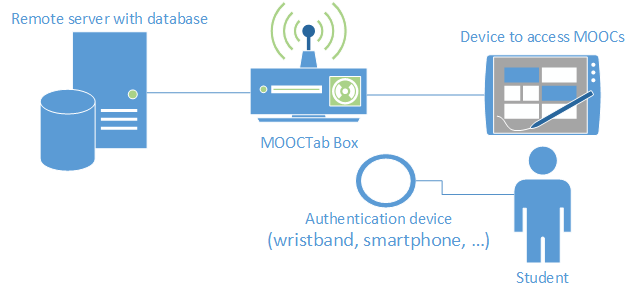
\includegraphics[]{ecosystem_mooctab}
	\caption{Écosytème MOOCTab}
\end{figure}

De plus, la solution comprend une MOOCBox qui permet aux utilisateurs de s'authentifier avec leurs badges et d'avoir accès au contenu qu'elle diffuse dans la salle de cours.
La MOOCBox est composée de deux éléments distincts, un serveur local à la salle de cours et un module \gls{nfc} permettant la partie authentification.

Le module \gls{nfc} de la box possède un élément sécurisé, qui permettra de stocker les données d'identification des étudiants. Ce module pourra lire les badges, les écrire et partager des informations avec l'autre partie de la box. C'est cette partie-là que NXP a la responsabilité de réaliser.

Notre partie de la box est composée d'une petite carte tournant sous Android à laquelle nous avons rattaché une puce \gls{nfc} avec son antenne. Mon rôle a été de réaliser la liaison entre la carte et la puce \gls{nfc}, autant au niveau matériel que logiciel.
\par
\begin{figure}
	\center
	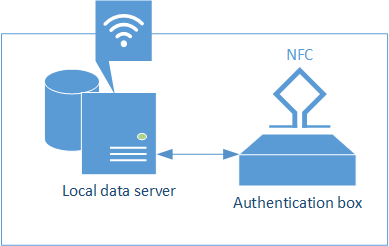
\includegraphics[]{moocbox_mooctab}
	\caption{Schéma conceptuel de la MOOCBox}
\end{figure}
Dans un premier temps il m'a été demandé de réaliser plusieurs démonstrations sous Android.
La première permettait d'accéder à un bracelet connecté qui agissait comme une carte étudiante. Il fallait pouvoir lire et écrire des informations dessus. Cette démonstration a été présentée à l'occasion d'un salon auquel NXP participait.

Afin de réaliser cette démonstration il m'a fallu apprendre comment fonctionnait une carte d'identification et comment elle était créée. Il a aussi fallu que j'apprenne à accéder au contenu du bracelet pour le lire et le modifier. J'ai ainsi découvert les avantages et les limitations du système.

La seconde venait compléter cette démonstration, il fallait pouvoir démontrer qu'il était possible d'accéder à l'élément sécurisé du lecteur (l'appareil Android) afin de traiter les informations qu'envoyait la carte (le bracelet).

Pour que cette démonstration puisse voir le jour nous avions à disposition des smartphones de référence qui servent de testeurs. Ayant un accès complet à ces smartphones avec les clés permettant d'accéder à l'élément sécurisé, nous avons pu y installer une petite application nommée loopback. Cette application permettait, entre autres, de renvoyer, sous forme inversée, les données que nous lui envoyons. Par exemple aabbcc était envoyé et loopback retournait ccbbaa.

Ces deux démonstrations ont été l'occasion pour moi d'apprendre à utiliser différentes manières de manipuler la \gls{nfc} sous Android.
\begin{figure}
	\center
	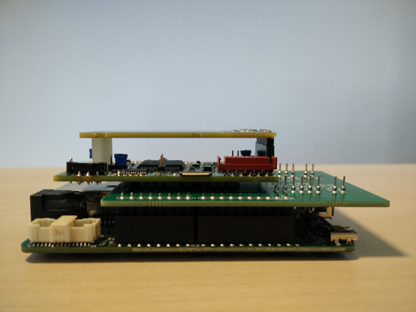
\includegraphics[]{demonstrateur}
	\caption{Photo du démonstrateur sans le câblage}
\end{figure}
La mission sur laquelle je travaille actuellement est la réalisation d'un démonstrateur qui sera notre partie de la MOOCbox.
Pour réaliser ce démonstrateur, il m'a fallu acquérir de nouvelles connaissances et comprendre les schémas électriques de la carte électronique que nous utilisons pour la puce \gls{nfc}. J'ai aussi dû étudier les plans de la carte Android, afin de faire les bons branchements, et apprendre à regénérer une image Android, afin d’y intégrer les pilotes, tout ceci dans le but de relier les deux cartes ensemble.

C'est pour moi une expérience inédite n'ayant jamais réalisé ce genre de tâches auparavant.

\section{NFC Playbook}
Il arrive que l'entreprise ait des besoins ponctuels de produire des démonstrations ou des modèles pour promouvoir l'utilisation de la \gls{nfc}, notamment dans les applications mobiles.
Récemment un collègue d'un autre service est venu solliciter mes compétences en la matière afin de développer un petit squelette de code pouvant être réutilisé.

Le but était de produire une petite application Android permettant d'héberger des mini-applications qui utiliseraient la \gls{nfc}. Il fallait avoir la possibilité de lancer les mini-applications, soit en cliquant dessus, soit en utilisant un tag \gls{nfc}.

Cette application sera utilisée lors d'un évènement du Dôme \cite{website:ledome} qui aura lieu les 16 et 17 février 2018. C'est un atelier qui se fera sur une journée et sera centré sur le thème du livre et des interactions numériques. Les développeurs et artistes de chaque équipe devront fabriquer des prototypes de livres améliorés grâce à l'outil numérique.

Cette mission m'a permis de faire une coupure par rapport au MOOCTab, tout en aidant un collègue. De plus ma contribution a permis d'éviter le recours à un prestataire et a donc induit des économies non négligeables.
\chapter{Évolution}
Lorsque je suis arrivée chez NXP la première fois je n'avais aucune expérience en entreprise. J'ai commencé par un stage de douze semaines, me permettant de faire mes premiers pas dans le monde professionnel et de trouver mon poste d'apprentie.
Cela fait maintenant deux ans et demi que j'évolue au fil des mois autant en entreprise qu'à l'école.
\section{Savoir-faire}
Les premières évolutions notables sont au niveau technique. J'ai abordé de nouvelles technologies, appris des langages que je ne connaissais pas, et assimilé de nouvelles compétences.
Lors de mon entrée en entreprise j'avais des connaissances dans quelques langages de programmation, avec une préférence pour les langages web, sans vraiment avoir pu approfondir la plupart d'entre eux.

J'ai été recrutée pour travailler sur des projets faisant l'emploi de la \gls{nfc}, principalement du développement mobile sous Android, mais pas uniquement.

Mes premières missions ont consisté à de la maintenance et du support sur des projets existants, Smartcampus et LabTab. Cela m'a permis de progresser sur les langages JEE et Java pour Android. J'ai aussi pu appliquer des compétences en base de données ainsi qu'en installation et gestion de serveur.

Avec le temps, mes tâches ont évolué. On m'a confié de nouveaux projets à réaliser de A à Z.
Mon premier projet était un service de report d'incidents. Des tags \gls{nfc} permettaient de simplifier le remplissage d'informations concernant l'endroit où se situait l'incident.

Bien que le développement Android fût indispensable pour la partie mobile, j'avais le choix pour les technologies utilisées pour le reste. J'ai alors décidé de me former sur une technologie que je ne connaissais pas, Spring, ceci tout en continuant d'appliquer ce que j'avais déjà acquis.

Finalement c'est sur le projet MOOCTab, qui a occupé la majeure partie de mon temps, que j'ai gagné le plus en compétences. J'ai dû réaliser plusieurs démonstrateurs sous Android avec des bracelets connectés notamment.
Au-delà de l'aspect technologique sous Android, j'avais envie d'améliorer mes compétences et ma productivité, c'est pourquoi j'ai décidé de commencer à utiliser Kotlin. Il m'a été facile d'apprendre ce langage car il ressemble beaucoup au Scala que nous avons pu aborder en cours. 

Jusqu'alors je n'avais travaillé que sur de simple tags \gls{nfc}. Les bracelets remplaçaient l'utilisation de cartes pour s'identifier voire s'authentifier.
La gestion de cartes en \gls{nfc} est un système flexible mais néanmoins particulier. Il est possible de créer une carte vide sur les bracelets, à l'aide d'une simple application Android qui se sert de la connexion en Bluetooth. Par contre, si l'on souhaite la personnaliser en ajoutant du chiffrement, il est nécessaire d'avoir recours à un serveur distant contenant les clés d'auhentification.

J'ai donc découvert de toutes nouvelles technologies et concepts qui ne ressemblaient à rien de ce que j'avais pu faire.
\par
Dans cet ensemble de nouveautés on peut citer :
\begin{itemize}
\item \gls{mifare} \gls{desfire}, pour la création de cartes;
\item La compilation de sources Android;
\item L'étude des schémas électriques, qui ajoute un apport de connaissances en électroniques.
\end{itemize}

\par

C'est sans aucun doute le projet MOOCTab qui a été pour moi la clé d'une forte évolution technique.
\section{Savoir-être}
Ces projets ne m'ont pas uniquement permis de gagner en technicité mais aussi sur d'autres compétences.
Malgré le fait que je n'avais aucun problème à travailler en autonomie, j'avais besoin de beaucoup d'appui lors de mes débuts. Je manquais beaucoup de confiance en moi et en ce que j'étais capable de faire.

Petit à petit et avec l'aide de mes maîtres d'apprentissage j'ai su surmonter mes difficultés.
Et au fil des projets, sans m'en rendre compte j'ai pris confiance en moi, ce qui a résulté en plus de prises d'initiatives et en propositions de solutions.

Le travail en autonomie et la réalisation de divers projets m'a aussi permis d'améliorer ma gestion du temps et du stress.

\subsection{Collaboration}
J'ai beaucoup travaillé en autonomie sur les diverses missions qui m'ont été attribuées. Je n'ai pu expérimenter le travail en équipe qu'au travers de projets à l'ENSICAEN.

En revanche, j'ai appris à solliciter d'autres professionnels lorsque cela était nécessaire.
En effet, pour le MOOCTab par exemple, j'ai dû demander des informations à d'autres collègues n'ayant pas moi-même les compétences spécifiques nécessaires.
J'ai aussi dû requérir de l'aide sur des tâches qui n'étaient pas de mon ressort comme du soudage de composants.

Dans le cadre du MOOCTab j'ai eu l'occasion de travailler avec d'autres entreprises. Il était important d'échanger des informations pour pouvoir intégrer le travail de chacun afin d'obtenir un produit final cohérent.

\chapter{Bilan}
L'écriture de ce rapport a été l'occasion de prendre du recul sur les trois dernières années, et plus particulièrement les derniers mois.
Le projet intensif organisé au Dôme m'a permis de me rendre compte de l'évolution de mes compétences.
En effet rencontrer des étudiants de la filière classique m'a fait prendre conscience de l'avantage de l'apprentissage. Grâce à l'expérience acquise en entreprise il est plus facile de mettre en application nos connaissances.

C'est sur cette dernière année que j'ai, à mon avis, le plus progressé.
Les changements de maîtres d'apprentissage ont contribué à cette progression. En effet ce n'est que récemment que la situation s'est réellement stabilisée. Pendant la période de transition, j'ai beaucoup été en autonomie, ce qui m'a forcé à m'adapter.

L'alternance de périodes école et entreprise permet de prendre du recul sur les unes comme sur les autres. En entreprise, on peut appliquer ce qui a été appris en cours et consolider nos connaissances. Les cours permettent eux avoir une vision critique de ce qui a été réalisé en entreprise tout en acquerrant de nouvelles connaissances. Cela m'a permis de porter un regard nouveau autant sur le monde du travail que sur mon avenir.

Ces trois années m'ont ainsi permis d'évoluer, autant en savoir-être qu'en savoir-faire, et m'ont donné les clés nécessaires pour continuer dans la vie active.

\chapter{Conclusion}
Le projet MOOCTab a bien avancé dernièrement.
La partie tablette Android est achevée, et pour la box les schémas de câblage sont terminés. Nous avons un début de démonstrateur, en plus des démonstrations sous Android.
L'avenir semble prometteur et nous sommes parfaitement dans les temps, le projet se terminant fin juin 2018.
Il reste à construire une image, pour la box, qui nous permette d'accéder à l'élément sécurisé de notre puce \gls{nfc}.

Dans la même veine, je serai amenée à développer une ou plusieurs applets qui tourneront sur un élément sécurisé. Que ce soit dans le cadre du MOOCTab ou en dehors.

Suite à mon travail sur le NFC Playbook, il est possible qu'on me redemande ce genre de missions à l'avenir.

Les derniers mois en entreprises s'annoncent intéressants avec les perspectives de nouveaux développements.

\printglossary[title={Glossaire}]

\bibliography{mybib}{}
\bibliographystyle{plain}
	
\end{document}


